% Options for packages loaded elsewhere
\PassOptionsToPackage{unicode}{hyperref}
\PassOptionsToPackage{hyphens}{url}
%
\documentclass[
]{article}
\usepackage{lmodern}
\usepackage{amssymb,amsmath}
\usepackage{ifxetex,ifluatex}
\ifnum 0\ifxetex 1\fi\ifluatex 1\fi=0 % if pdftex
  \usepackage[T1]{fontenc}
  \usepackage[utf8]{inputenc}
  \usepackage{textcomp} % provide euro and other symbols
\else % if luatex or xetex
  \usepackage{unicode-math}
  \defaultfontfeatures{Scale=MatchLowercase}
  \defaultfontfeatures[\rmfamily]{Ligatures=TeX,Scale=1}
\fi
% Use upquote if available, for straight quotes in verbatim environments
\IfFileExists{upquote.sty}{\usepackage{upquote}}{}
\IfFileExists{microtype.sty}{% use microtype if available
  \usepackage[]{microtype}
  \UseMicrotypeSet[protrusion]{basicmath} % disable protrusion for tt fonts
}{}
\makeatletter
\@ifundefined{KOMAClassName}{% if non-KOMA class
  \IfFileExists{parskip.sty}{%
    \usepackage{parskip}
  }{% else
    \setlength{\parindent}{0pt}
    \setlength{\parskip}{6pt plus 2pt minus 1pt}}
}{% if KOMA class
  \KOMAoptions{parskip=half}}
\makeatother
\usepackage{xcolor}
\IfFileExists{xurl.sty}{\usepackage{xurl}}{} % add URL line breaks if available
\IfFileExists{bookmark.sty}{\usepackage{bookmark}}{\usepackage{hyperref}}
\hypersetup{
  pdftitle={Trabajo práctico N°1: Búsqueda y Optimización},
  pdfauthor={Gino Avanzini; Emiliano Cabrino; Adrián Cantaloube; Gonzalo Fernández},
  hidelinks,
  pdfcreator={LaTeX via pandoc}}
\urlstyle{same} % disable monospaced font for URLs
\usepackage{color}
\usepackage{fancyvrb}
\newcommand{\VerbBar}{|}
\newcommand{\VERB}{\Verb[commandchars=\\\{\}]}
\DefineVerbatimEnvironment{Highlighting}{Verbatim}{commandchars=\\\{\}}
% Add ',fontsize=\small' for more characters per line
\newenvironment{Shaded}{}{}
\newcommand{\AlertTok}[1]{\textcolor[rgb]{1.00,0.00,0.00}{\textbf{#1}}}
\newcommand{\AnnotationTok}[1]{\textcolor[rgb]{0.38,0.63,0.69}{\textbf{\textit{#1}}}}
\newcommand{\AttributeTok}[1]{\textcolor[rgb]{0.49,0.56,0.16}{#1}}
\newcommand{\BaseNTok}[1]{\textcolor[rgb]{0.25,0.63,0.44}{#1}}
\newcommand{\BuiltInTok}[1]{#1}
\newcommand{\CharTok}[1]{\textcolor[rgb]{0.25,0.44,0.63}{#1}}
\newcommand{\CommentTok}[1]{\textcolor[rgb]{0.38,0.63,0.69}{\textit{#1}}}
\newcommand{\CommentVarTok}[1]{\textcolor[rgb]{0.38,0.63,0.69}{\textbf{\textit{#1}}}}
\newcommand{\ConstantTok}[1]{\textcolor[rgb]{0.53,0.00,0.00}{#1}}
\newcommand{\ControlFlowTok}[1]{\textcolor[rgb]{0.00,0.44,0.13}{\textbf{#1}}}
\newcommand{\DataTypeTok}[1]{\textcolor[rgb]{0.56,0.13,0.00}{#1}}
\newcommand{\DecValTok}[1]{\textcolor[rgb]{0.25,0.63,0.44}{#1}}
\newcommand{\DocumentationTok}[1]{\textcolor[rgb]{0.73,0.13,0.13}{\textit{#1}}}
\newcommand{\ErrorTok}[1]{\textcolor[rgb]{1.00,0.00,0.00}{\textbf{#1}}}
\newcommand{\ExtensionTok}[1]{#1}
\newcommand{\FloatTok}[1]{\textcolor[rgb]{0.25,0.63,0.44}{#1}}
\newcommand{\FunctionTok}[1]{\textcolor[rgb]{0.02,0.16,0.49}{#1}}
\newcommand{\ImportTok}[1]{#1}
\newcommand{\InformationTok}[1]{\textcolor[rgb]{0.38,0.63,0.69}{\textbf{\textit{#1}}}}
\newcommand{\KeywordTok}[1]{\textcolor[rgb]{0.00,0.44,0.13}{\textbf{#1}}}
\newcommand{\NormalTok}[1]{#1}
\newcommand{\OperatorTok}[1]{\textcolor[rgb]{0.40,0.40,0.40}{#1}}
\newcommand{\OtherTok}[1]{\textcolor[rgb]{0.00,0.44,0.13}{#1}}
\newcommand{\PreprocessorTok}[1]{\textcolor[rgb]{0.74,0.48,0.00}{#1}}
\newcommand{\RegionMarkerTok}[1]{#1}
\newcommand{\SpecialCharTok}[1]{\textcolor[rgb]{0.25,0.44,0.63}{#1}}
\newcommand{\SpecialStringTok}[1]{\textcolor[rgb]{0.73,0.40,0.53}{#1}}
\newcommand{\StringTok}[1]{\textcolor[rgb]{0.25,0.44,0.63}{#1}}
\newcommand{\VariableTok}[1]{\textcolor[rgb]{0.10,0.09,0.49}{#1}}
\newcommand{\VerbatimStringTok}[1]{\textcolor[rgb]{0.25,0.44,0.63}{#1}}
\newcommand{\WarningTok}[1]{\textcolor[rgb]{0.38,0.63,0.69}{\textbf{\textit{#1}}}}
\usepackage{graphicx,grffile}
\makeatletter
\def\maxwidth{\ifdim\Gin@nat@width>\linewidth\linewidth\else\Gin@nat@width\fi}
\def\maxheight{\ifdim\Gin@nat@height>\textheight\textheight\else\Gin@nat@height\fi}
\makeatother
% Scale images if necessary, so that they will not overflow the page
% margins by default, and it is still possible to overwrite the defaults
% using explicit options in \includegraphics[width, height, ...]{}
\setkeys{Gin}{width=\maxwidth,height=\maxheight,keepaspectratio}
% Set default figure placement to htbp
\makeatletter
\def\fps@figure{htbp}
\makeatother
\setlength{\emergencystretch}{3em} % prevent overfull lines
\providecommand{\tightlist}{%
  \setlength{\itemsep}{0pt}\setlength{\parskip}{0pt}}
\setcounter{secnumdepth}{-\maxdimen} % remove section numbering

\title{Trabajo práctico N°1: Búsqueda y Optimización}
\author{Gino Avanzini \and Emiliano Cabrino \and Adrián Cantaloube \and Gonzalo Fernández}
\date{}

\begin{document}
\maketitle

\hypertarget{anuxe1lisis-y-selecciuxf3n-de-algoritmos-seguxfan-el-tipo-de-problema}{%
\section{Análisis y selección de algoritmos según el tipo de
problema}\label{anuxe1lisis-y-selecciuxf3n-de-algoritmos-seguxfan-el-tipo-de-problema}}

En los problemas enunciados abajo - Qué algoritmo/s utilizaría en cada
caso. Justifique. - Defina el problema (estado inicial, modelo de
transición, prueba de meta, funciones heurísticas si aplican, función de
costo/calidad) - Estime la complejidad del problema y del algoritmo

\hypertarget{diseuxf1o-de-un-proceso-de-manufactura}{%
\subsection{Diseño de un proceso de
manufactura}\label{diseuxf1o-de-un-proceso-de-manufactura}}

Es un problema de satisfacción de restricciones: necesitamos encontrar
el plan de manufactura. La resolución del problema nos permite crear
dicho plan describiendo un estado inicial y un objetivo, siendo ambos
fijados por el encargado de la manufactura, y las tareas que se podrán
llevar a cabo. Un estado está definido por el instante de tiempo en que
cada tarea debe comenzar a realizarse. Cada tarea lleva consigo
precondiciones que se deberán cumplir para que esta tarea se lleve a
cabo y el planificador deberá diseñar el plan para que la manufactura
sea correcta y lo mas fluida posible describiendo el modelo de
transición. Al finalizar el algoritmo se calcularán costos de dinero y
tiempo de manufactura y se comprobará si la planificación cumple con las
expectativas. De otra forma se deberá reconstruir para buscar una mejor
solución.

Para encontrar la solución podemos recurrir a algoritmos genéticos o a
un algoritmo como el de backtracking.

\hypertarget{planificaciuxf3n-de-uxf3rdenes-de-fabricaciuxf3n}{%
\subsection{Planificación de órdenes de
fabricación}\label{planificaciuxf3n-de-uxf3rdenes-de-fabricaciuxf3n}}

Es un problema de planificación. Cuando las empresas trabajan con
pedidos es común que estos lleguen todos los días de forma
desorganizada. Es necesario agruparlos para que la producción se lleve a
cabo de forma simultánea. Por ejemplo: llegaron pedidos de un mismo
modelo, de clientes diferentes, ellos pueden ser cortados y fabricados
al mismo tiempo. Con ese agrupamiento se estará elaborando una única
orden de fabricación. Ahorrando tiempo al evitar un seccionamiento
innecesario.

El orden del plan y el ahorro a la hora de planificar se pueden basar
según el valor de facturación o según el plazo y cantidad de productos.

Para poder resolver este problema podemos usar un algoritmo de temple
simulado. Un estado sería una asignación completa de tiempos en los que
deben comenzar los procesos de manufactura de cada orden. Además
verificamos que las asignaciones sean válidas mediante algoritmos de
consistencia de arco y nodo. Como función de energía se puede tener en
cuenta el tiempo total de ejecución de todas las órdenes, los tiempos
muertos, etc. Se buscaría minimizar esta función de energía, premiando
los trabajos que se realizan en paralelo y penando aquellas asignaciones
que implican mayor tiempo total de ejecución.

\hypertarget{encontrar-la-ubicaciuxf3n-uxf3ptima-de-aerogeneradores-en-un-parque-euxf3lico}{%
\subsection{Encontrar la ubicación óptima de aerogeneradores en un
parque
eólico}\label{encontrar-la-ubicaciuxf3n-uxf3ptima-de-aerogeneradores-en-un-parque-euxf3lico}}

Es un problema de optimización: Se busca maximizar la energía generada
por un determinado número de aerogeneradores en un campo eólico dada la
información sobre el viento en la zona. Para lograrlo hay que determinar
la mejor disposición de los generadores en el parque.

La resolución del problema se puede encasillar dentro de la familia de
algoritmos de búsqueda continua. Además se puede discretizar el espacion
y convertir el problema a uno de búsqueda clásico. Entre ellos se
encuentran, por ejemplo, los algoritmos genéticos y de recocido
simulado. El estado inicial del problema es obtener un configuración
aleatoria de los generadores en el espacio del campo. El modelo de
transición consiste en reubicar alguno de los aerogeneradores en otra
posición del campo y proseguir con el algoritmo, evaluando si el nuevo
estado produce una mejora o no con la función objetivo.

La función de energía (en el caso del temple) es una función que dada la
información del viento en la zona, valora qué tan buena es la
distribución de generadores. Para generar estados vecinos se puede
reubicar cierta cantidad de generadores y evaluar la nueva
configuración.

Además, si se quisiera, se podría fraccionar el campo eólico en sectores
y hacer optimizaciones locales en esos sectores. De esta forma se podría
paralelizar el problema y obtener una solución más rápidamente.

\hypertarget{planificar-trayectorias-de-un-brazo-robuxf3tico-con-6-grados-de-libertad}{%
\subsection{Planificar trayectorias de un brazo robótico con 6 grados de
libertad}\label{planificar-trayectorias-de-un-brazo-robuxf3tico-con-6-grados-de-libertad}}

Es un problema de planificación y/o optimización: Se busca una
combinación entre ambas, planificación para conocer las acciones que
debe tomar, y optimización para llegar del estado inicial al final con
el menor gasto posible. Ambas nos ayudarán a tomar decisiones en tiempo
real ya que trabajan en conjunto.

El estado inicial y final son descriptas por el operario y no generadas
aleatoriamente. Con el modelo de transición vemos el movimiento de los
eslabones del robot para llegar al próximo estado (punto discretizado de
la trayectoria). Podríamos usar la heurística del ejercicio 2)a de este
práctico (A*) para llegar al objetivo. En este caso no podríamos usar
algoritmos de búsqueda local ya que no solo debemos llegar al estado
final, sino que necesitamos seguir una trayectoria establecida.

\hypertarget{diseuxf1o-de-un-generador}{%
\subsection{Diseño de un generador}\label{diseuxf1o-de-un-generador}}

Los problemas de diseño generalmente son de optimización. Esto significa
que debemos encontrar la forma de diseñar el generador maximizando el
ahorro de recursos y el rendimiento del mismo. Para que el generador
cumpla con las especificaciones deseadas, habrá que implementar un
algoritmo relacionando las propiedades y cantidades de los materiales a
utilizar para saber que tanta eficiencia aportarán al generador. La
combinación mas optima es la que utilizaremos como meta.

Para la resolución de este problema podemos utilizar un algoritmo
genético. Cada individuo estaría caracterizado por, por ejemplo,
cantidad de polos del rotor, tipo de polos, cantidad de vueltas por
bobina, material del núclo del estator y el rotor, potencia de salida,
etc. Para cada configuración habrá un valor de fitness que será función
del costo de construcción, rendimiento estimado y peso, entre otros.

\hypertarget{definiciuxf3n-de-una-secuencia-de-ensamblado-uxf3ptima}{%
\subsection{Definición de una secuencia de ensamblado
óptima}\label{definiciuxf3n-de-una-secuencia-de-ensamblado-uxf3ptima}}

Es un problema de búsqueda. Se quiere encontrar la secuencia óptima de
partes a colocar en, por ejemplo, una placa electrónica.

Para esto podríamos utilizar un algoritmo como el A* en el cual partimos
de un componente inicial y queremos buscar la mejor secuencia para
colocar todos los componentes, considerando que puede haber varios
unidades del mismo tipo en distintos lugares de la placa.

La heurística sería la distancia en línea recta entre un componente y
otro. El costo aumenta al realizar cada viaje a un punto de la placa y
al realizar un cambio en el tipo de componente.

Dado que buscamos optimalidad con un A* obtendremos la mejor secuencia.

\hypertarget{planificaciuxf3n-del-proyecto-de-una-obra}{%
\subsection{Planificación del proyecto de una
obra}\label{planificaciuxf3n-del-proyecto-de-una-obra}}

Es un problema de planificación. Se busca encontrar un orden en las
tareas a realizar (algunas de forma paralela o simultanea) de manera que
se cumplan los ordenes de precedencia de cada una de ellas. Se inicia
con las tareas de la obra que no requieren requisitos previos para ser
ejecutadas. Se procederá con las tareas que requieran la finalización de
la/s primera/s y así sucesivamente hasta concluir la obra. Cada tarea
conlleva cierto tiempo, parámetro que utilizaremos para calcular las
ganancias y estimar el rango de tiempo que nos llevará a cabo realizar
la obra.

Se puede utilizar un algoritmo de backtracking junto con un algoritmo
para verificación la consistencia de las asignaciones (AC3, etc.)

\hypertarget{implementaciuxf3n-de-algoritmo-a-para-trayectoria-de-robot-de-6-grados-de-libertad}{%
\section{Implementación de algoritmo A* para trayectoria de robot de 6
grados de
libertad}\label{implementaciuxf3n-de-algoritmo-a-para-trayectoria-de-robot-de-6-grados-de-libertad}}

El problema del robot con 6 grados de libertad fue modelado en el
espacio articular, donde cada estado del problema es el valor angular de
cada articulación con una discretización de ángulos sexagecimales
enteros, es decir, un vector de estado es una lista de 6 componentes
enteros.

La función heurística adoptada en el modelo es la raíz cuadrada de la
suma del cuadrado de cada componente, distancia euclidiana del espacio
de estados, desde el estado en cuestión al estado objetivo.

El estado inicial es sencillamente la configuración inicial del brazo
robótico. La prueba de meta es la comprobación de si el estado actual es
igual al estado objetivo, es decir, comprobar si el valor angular de
cada articulación es igual el objetivo.

\hypertarget{anuxe1lisis-de-tiempo-de-ejecuciuxf3n-del-algoritmo-en-funciuxf3n-de-la-cantidad-de-grados-de-libertad}{%
\subsection{Análisis de tiempo de ejecución del algoritmo en función de
la cantidad de grados de
libertad}\label{anuxe1lisis-de-tiempo-de-ejecuciuxf3n-del-algoritmo-en-funciuxf3n-de-la-cantidad-de-grados-de-libertad}}

El tiempo de ejecución del algoritmo se incrementa al aumentar la
cantidad de grados de libertad del espacio articular del sistema. A
continuación se analiza de 2 a 6 grados de libertad.

\begin{Shaded}
\begin{Highlighting}[]
\ImportTok{from}\NormalTok{ time }\ImportTok{import}\NormalTok{ time}
\end{Highlighting}
\end{Shaded}

\begin{Shaded}
\begin{Highlighting}[]
\ImportTok{from}\NormalTok{ a_star2b }\ImportTok{import}\NormalTok{ Node, a_star}
\ImportTok{from}\NormalTok{ a_star2a }\ImportTok{import}\NormalTok{ generate_neighbours, obstaculos}
\end{Highlighting}
\end{Shaded}

Los parámetros TOP y STEP están definidos en el archivo
\href{./a_star2a.py}{a\_star2a.py}.

\begin{Shaded}
\begin{Highlighting}[]
\NormalTok{TOP }\OperatorTok{=} \DecValTok{50}
\NormalTok{STEP }\OperatorTok{=} \DecValTok{10}
\end{Highlighting}
\end{Shaded}

\begin{Shaded}
\begin{Highlighting}[]
\NormalTok{register }\OperatorTok{=}\NormalTok{ []}

\NormalTok{i }\OperatorTok{=} \DecValTok{2}
\ControlFlowTok{while}\NormalTok{ (i }\OperatorTok{<=} \DecValTok{6}\NormalTok{):}
    
\NormalTok{    GDL }\OperatorTok{=}\NormalTok{ i}
    
\NormalTok{    initial_state }\OperatorTok{=}\NormalTok{ GDL }\OperatorTok{*}\NormalTok{ [}\DecValTok{0}\NormalTok{]}
\NormalTok{    start }\OperatorTok{=}\NormalTok{ Node(initial_state)}

\NormalTok{    end_state }\OperatorTok{=}\NormalTok{ GDL }\OperatorTok{*}\NormalTok{ [TOP]}
\NormalTok{    goal }\OperatorTok{=}\NormalTok{ Node(end_state)}
    
    \CommentTok{# wall = obstaculos(GDL)}
    \CommentTok{# wall = None}
    
\NormalTok{    t_start }\OperatorTok{=}\NormalTok{ time()}
    \CommentTok{# ans = a_star(start, goal, generate_neighbours, wall=wall)}
\NormalTok{    ans }\OperatorTok{=}\NormalTok{ a_star(start, goal, generate_neighbours, dim}\OperatorTok{=}\NormalTok{GDL)}

    \ControlFlowTok{if}\NormalTok{ ans[}\DecValTok{1}\NormalTok{]:}
\NormalTok{        t_end }\OperatorTok{=}\NormalTok{ time()}
\NormalTok{        register.append(t_end }\OperatorTok{-}\NormalTok{ t_start)}
\NormalTok{        i }\OperatorTok{+=} \DecValTok{1}
\end{Highlighting}
\end{Shaded}

\begin{verbatim}
1555960528.8629613
2
1555960528.8864892
3
1555960529.4057345
4
1555960551.4310658
5
1555961599.8360023
6
\end{verbatim}

\begin{Shaded}
\begin{Highlighting}[]
\ImportTok{from}\NormalTok{ matplotlib }\ImportTok{import}\NormalTok{ pyplot }\ImportTok{as}\NormalTok{ plt}
\end{Highlighting}
\end{Shaded}

\begin{Shaded}
\begin{Highlighting}[]
\BuiltInTok{print}\NormalTok{(register)}
\end{Highlighting}
\end{Shaded}

\begin{verbatim}
[0.0005648136138916016, 0.02310776710510254, 0.5191671848297119, 22.02523684501648, 1048.4048516750336]
\end{verbatim}

\begin{Shaded}
\begin{Highlighting}[]
\NormalTok{gdl }\OperatorTok{=}\NormalTok{ [}\DecValTok{2}\NormalTok{, }\DecValTok{3}\NormalTok{, }\DecValTok{4}\NormalTok{, }\DecValTok{5}\NormalTok{, }\DecValTok{6}\NormalTok{]}
\NormalTok{plt.plot(gdl, register)}
\NormalTok{plt.grid()}
\end{Highlighting}
\end{Shaded}

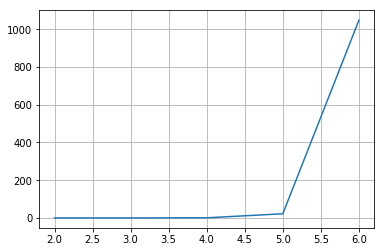
\includegraphics{output_11_0.png}

Si se analiza el tiempo de ejecución en relación del tiempo de ejecución
máximo, es decir para 6 grados de libertad, los resultados son los
siguientes:

\begin{Shaded}
\begin{Highlighting}[]
\ControlFlowTok{for}\NormalTok{ i }\KeywordTok{in}\NormalTok{ register:}
    \BuiltInTok{print}\NormalTok{(i }\OperatorTok{/}\NormalTok{ register[}\BuiltInTok{len}\NormalTok{(register)}\OperatorTok{-}\DecValTok{1}\NormalTok{])}
\end{Highlighting}
\end{Shaded}

\begin{verbatim}
5.387361695142868e-07
2.2040881505062974e-05
0.0004951972360679559
0.02100833166674765
1.0
\end{verbatim}

\hypertarget{conclusiuxf3n}{%
\subsection{Conclusión}\label{conclusiuxf3n}}

Para observar el crecimiento exponencial, se muestra cuánto más grande
es un tiempo de ejecución con relación al tiempo para un grado de
libertad menos:

\begin{Shaded}
\begin{Highlighting}[]
\ControlFlowTok{for}\NormalTok{ i }\KeywordTok{in} \BuiltInTok{range}\NormalTok{(}\DecValTok{0}\NormalTok{, }\BuiltInTok{len}\NormalTok{(register)}\OperatorTok{-}\DecValTok{1}\NormalTok{):}
    \BuiltInTok{print}\NormalTok{(register[i}\OperatorTok{+}\DecValTok{1}\NormalTok{]}\OperatorTok{/}\NormalTok{register[i])}
\end{Highlighting}
\end{Shaded}

\begin{verbatim}
40.912199240185736
22.467215567317712
42.42416987938252
47.600162443304214
\end{verbatim}

Se puede observar que incrementar en 1 la dimensión del espacio
articular del robot implica escalar aproximadamente en 40 el tiempo de
ejecución del programa.

La complejidad del algoritmo A* es O(b\^{}d) siendo b la cantidad de
estados vecinos y d el factor de ramificación o profundidad.

Por lo tanto, para reducir el tiempo de ejecución debería modificarse la
generación de estados vecinos aumentando su cantidad, y así obtener un
árbol de estados más ancho pero de menor profundidad.

\hypertarget{implementaciuxf3n-de-algoritmo-a-para-calcular-camino-muxe1s-corto-entre-dos-posiciones-de-un-almacen}{%
\section{Implementación de algoritmo A* para calcular camino más corto
entre dos posiciones de un
almacen}\label{implementaciuxf3n-de-algoritmo-a-para-calcular-camino-muxe1s-corto-entre-dos-posiciones-de-un-almacen}}

El problema del camino más corto entre dos posiciones de un almacen con
un determinado layout, se modeló de tal forma que cada estado es una
posición del almacén en coordenadas rectangulares. Estas coordenadas son
tales que el (0, 0) se encuentra en la esquina superior izquierda, y x e
y crecen hacia la derecha y abajo respectivamente.

La función heurística adoptada en el modelo es la raíz cuadrada de la
suma del cuadrado de cada componente, distancia euclidiana del espacio
de estados, desde el estado en cuestión al estado objetivo. Esto debido
a que ya se encontraba implementado en el ejercicio anteriror.

El estado inicial es la posición inicial, por ejemplo (0, 0), y el
estado final la posición objetivo. Se consideran posiciones válidas
únicamente los pasillos, por lo que la posición de una determinada
estantería o producto es ubicado estando en el pasillo frente a éste.

El algoritmo se implementó separando las funciones independientes del
modelado del problema de las dependientes de éste. Por lo tanto aquellas
funciones propias del algoritmo A* pudieron reutilizarse sin
inconvenientes en ambos ejercicios sin necesidad de una nueva
implementación. Para información más específica consultar documentación
del código.

\hypertarget{implementaciuxf3n-de-recocido-simulado-para-optimizaciuxf3n-de-orden-de-picking-en-almacen}{%
\section{Implementación de recocido simulado para optimización de orden
de picking en
almacen}\label{implementaciuxf3n-de-recocido-simulado-para-optimizaciuxf3n-de-orden-de-picking-en-almacen}}

En este problema el objetivo es determinar el orden óptimo de picking
para una serie de productos en el almacén. Esto se determina mediante un
algoritmo de recocido simulado cuyos parámetros e implementación se
explicarán a continuación.

\hypertarget{anuxe1lisis-del-algoritmo}{%
\subsection{Análisis del algoritmo}\label{anuxe1lisis-del-algoritmo}}

El algoritmo de recocido simulado tiene varios parámetros que afectan
los resultados. A continuación hablaremos brevemente de los mismos.

\begin{itemize}
\tightlist
\item
  Perfil de decrecimiento de temperatura
\end{itemize}

Como perfil de decrecimiento se eligió, por simplicidad y para evitar el
tuning de otro hiperparámetro, una función lineal en la que la
temperatura disminuye un grado por cada iteración.

\begin{itemize}
\tightlist
\item
  Temperatura inicial
\end{itemize}

Se evaluaron distintas temperaturas iniciales y se hizo un análisis en
el que se evalúa cuán mejor es la solución final que otorga el algoritmo
en comparación a la solución inicial. Dicho análisis se explica más
adelante pero la conclusión es que no existe una gran mejora en la
calidad de la solución con temperaturas iniciales mayores a 200.

\begin{itemize}
\tightlist
\item
  Energía
\end{itemize}

Como función de energía para obtener la calidad de la solución para cada
estado se utiliza el algoritmo A* ya implementado en el problema
anterior. Para cada secuencia de coordenadas que visitar, se calcula la
longitud del camino óptimo para ir de una coordenada a la siguiente
dentro de la secuencia. El valor de la energía del estado será la suma
de las distancias recorridas para ir de una coordenada a la otra,
comenzando y finalizando en {[}0, 0{]}.

\begin{itemize}
\tightlist
\item
  Generación de vecinos
\end{itemize}

Un estado en el algoritmo es una lista con una secuencia de coordenadas
que visitar. Para generar vecinos se seleccionan las posiciones de dos
elementos aleatorios dentro de la lista de coordenadas y se
intercambian. Luego se calcula la energía del estado vecino y este se
acepta siempre que tenga menor costo y cuando tenga mayor costo se
acepta con probabilidad exp(-delta/T).

\hypertarget{modelado-del-problema}{%
\subsection{Modelado del problema}\label{modelado-del-problema}}

El input del programa es una lista de productos que hay que ir a buscar
y como salida se obtiene el orden óptimo del picking para minimizar la
distancia recorrida. Antes de la ejecución en sí del temple, se realiza
una abstracción en la que se convierte de número de producto (o posición
en el almacén) a la coordenada cartesiana a la que hay que ir. Esto se
hace para poder reutilizar el algoritmo ya usado del A* y para, además,
poder usar a futuro este mismo código para el algoritmo genético.

Luego, a cada orden se le agregan dos coordenadas indicando que debe
partir y volver a un punto determinado del almacén el cual es, en
nuestro caso, {[}0, 0{]}. Así, por ejemplo, para ir a buscar los
productos 8, 6, 2, 14, 30 y 17 obtendremos algo así:

\begin{Shaded}
\begin{Highlighting}[]
\ImportTok{from}\NormalTok{ simulated_annealing }\ImportTok{import}\NormalTok{ map_to_coord, distance, temple_simulado, neighbours_annealing}
\end{Highlighting}
\end{Shaded}

La secuencia de coordenadas, con su respectiva energía, antes de la
ejecución del algoritmo es:

\begin{Shaded}
\begin{Highlighting}[]
\NormalTok{pos_pick }\OperatorTok{=}\NormalTok{ [}\DecValTok{8}\NormalTok{, }\DecValTok{6}\NormalTok{, }\DecValTok{2}\NormalTok{, }\DecValTok{14}\NormalTok{, }\DecValTok{30}\NormalTok{, }\DecValTok{17}\NormalTok{]}
\NormalTok{coordenadas }\OperatorTok{=}\NormalTok{ map_to_coord(pos_pick)}
\BuiltInTok{print}\NormalTok{(}\StringTok{"Estado inicial: "}\NormalTok{, coordenadas)}
\BuiltInTok{print}\NormalTok{(}\StringTok{"Energía: "}\NormalTok{, distance(coordenadas)) }\CommentTok{# Energía del estado inicial}
\end{Highlighting}
\end{Shaded}

\begin{verbatim}
Estado inicial:  [[0, 0], [6, 0], [4, 0], [2, 0], [9, 0], [9, 3], [1, 6], [0, 0]]
Energía:  40
\end{verbatim}

Y luego de la ejecución, la secuencia de coordenas con su respectiva
energía es:

\begin{Shaded}
\begin{Highlighting}[]
\NormalTok{T0 }\OperatorTok{=} \DecValTok{200}
\NormalTok{best_path }\OperatorTok{=}\NormalTok{ temple_simulado(coordenadas, T0, neighbours_annealing, distance)}

\BuiltInTok{print}\NormalTok{(}\StringTok{"Estado final: "}\NormalTok{, best_path[}\DecValTok{0}\NormalTok{])}
\BuiltInTok{print}\NormalTok{(}\StringTok{"Energía: "}\NormalTok{, best_path[}\DecValTok{1}\NormalTok{]) }\CommentTok{# Energía del estado inicial}
\end{Highlighting}
\end{Shaded}

\begin{verbatim}
Estado final:  [[0, 0], [2, 0], [4, 0], [6, 0], [9, 0], [9, 3], [1, 6], [0, 0]]
Energía:  32
\end{verbatim}

Primero se genera la secuencia de coordenadas a las que hay que ir para
buscar los productos tal como se dieron en la orden y el costo (en
pasos) de busar los productos en dicha secuencia. Al finalizar la
ejecución del algoritmo se devuelve la secuencia de coordenadas
``óptimas'' a las que hay que ir junto con el costo del nuevo camino.

La solución obtenida en el algoritmo no es la final que se obtendría con
el algoritmo vanilla sino la solución con mejor costo de todos los
estados generados. Como nuestro objetivo es optimizar el picking, lo
único que nos interesa es obtener el mejor resultado y no el último
obtenido.

Para calcular el costo de la secuencia se utiliza el algoritmo A* para
obtener el camino óptimo al pasar de la primera coordenada de la
secuencia a la segunda, de la segunda a la tercera y así sucesivamente.
En cada ejecución del A* se suma la distancia recorrida al ir de una
coordenada a la otra y la suma total será el costo de la secuencia dada.
Como vemos en el ejemplo dado, el costo del camino disminuyó de 40 a 32
pasos.

\hypertarget{anuxe1lisis-de-duraciuxf3n-de-la-ejecuciuxf3n-vs-cantidad-de-productos-en-una-orden-para-temperatura-inicial-constante}{%
\subsection{Análisis de duración de la ejecución vs cantidad de
productos en una orden para temperatura inicial
constante}\label{anuxe1lisis-de-duraciuxf3n-de-la-ejecuciuxf3n-vs-cantidad-de-productos-en-una-orden-para-temperatura-inicial-constante}}

En este análisis se ve la complejidad temporal del algoritmo en función
de la cantidad de productos que tenga una orden para temperatura inicial
constante. Así es que se calcula el tiempo de ejecución del algoritmo
para órdenes con 3, 5, 7, 10, 13, 15, 20, 25 y 30 productos. Para
eliminar las variaciones debido a la aleatoriedad en la generación de
las órdenes, se toma, para cada tamaño de orden (3, 5, 7, etc.) el
tiempo promedio de ejecución luego de 50 iteraciones. Esto es, se hace
un promedio de tiempo con 50 ejecuciones para cada tamaño de orden.

\begin{Shaded}
\begin{Highlighting}[]
\ImportTok{from}\NormalTok{ time }\ImportTok{import}\NormalTok{ time}
\ImportTok{from}\NormalTok{ random }\ImportTok{import}\NormalTok{ randint}
\end{Highlighting}
\end{Shaded}

\begin{Shaded}
\begin{Highlighting}[]
\NormalTok{ITER }\OperatorTok{=} \DecValTok{50}
\NormalTok{T0 }\OperatorTok{=} \DecValTok{200}

\CommentTok{# Cantidad de productos en una orden}
\NormalTok{inputs }\OperatorTok{=}\NormalTok{ [}\DecValTok{3}\NormalTok{, }\DecValTok{5}\NormalTok{, }\DecValTok{10}\NormalTok{, }\DecValTok{15}\NormalTok{, }\DecValTok{20}\NormalTok{, }\DecValTok{25}\NormalTok{, }\DecValTok{30}\NormalTok{]}

\NormalTok{time_exec }\OperatorTok{=}\NormalTok{ []}

\ControlFlowTok{for}\NormalTok{ i }\KeywordTok{in}\NormalTok{ inputs:}
\NormalTok{    time_avg }\OperatorTok{=} \DecValTok{0}
\NormalTok{    pos_pick }\OperatorTok{=}\NormalTok{ []}

    \ControlFlowTok{for}\NormalTok{ j }\KeywordTok{in} \BuiltInTok{range}\NormalTok{(}\DecValTok{0}\NormalTok{, ITER):}
\NormalTok{        pos_pick }\OperatorTok{=}\NormalTok{ [randint(}\DecValTok{0}\NormalTok{, }\DecValTok{31}\NormalTok{) }\ControlFlowTok{for}\NormalTok{ i }\KeywordTok{in} \BuiltInTok{range}\NormalTok{(}\DecValTok{0}\NormalTok{, i)]}

\NormalTok{        coordenadas }\OperatorTok{=}\NormalTok{ map_to_coord(pos_pick)}

\NormalTok{        start }\OperatorTok{=}\NormalTok{ time()}
\NormalTok{        _ }\OperatorTok{=}\NormalTok{ temple_simulado(coordenadas, T0, neighbours_annealing, distance)}
\NormalTok{        end }\OperatorTok{=}\NormalTok{ time()}

\NormalTok{        time_avg }\OperatorTok{+=}\NormalTok{ end }\OperatorTok{-}\NormalTok{ start}

\NormalTok{    time_avg }\OperatorTok{=}\NormalTok{ time_avg}\OperatorTok{/}\NormalTok{ITER}
\NormalTok{    time_exec.append(time_avg)}
\end{Highlighting}
\end{Shaded}

Se obtiene, como es de esperarse, un perfil lineal. Duplicar la cantidad
de productos en la orden implica duplicar el tiempo de ejecución.

\begin{Shaded}
\begin{Highlighting}[]
\ImportTok{from}\NormalTok{ matplotlib }\ImportTok{import}\NormalTok{ pyplot }\ImportTok{as}\NormalTok{ plt}
\end{Highlighting}
\end{Shaded}

\begin{Shaded}
\begin{Highlighting}[]
\NormalTok{plt.plot(time_exec)}
\NormalTok{plt.grid()}
\end{Highlighting}
\end{Shaded}

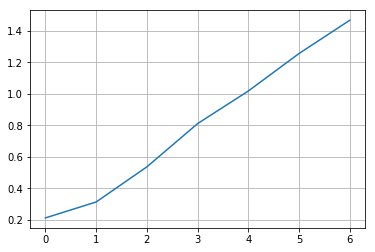
\includegraphics{output_18_0.png}

\hypertarget{anuxe1lisis-de-temperatura-inicial-cantidad-de-iteraciones-vs-mejora-en-la-soluciuxf3n}{%
\subsection{Análisis de temperatura inicial (cantidad de iteraciones) vs
mejora en la
solución}\label{anuxe1lisis-de-temperatura-inicial-cantidad-de-iteraciones-vs-mejora-en-la-soluciuxf3n}}

Luego, se hizo el análisis de mejora en la solución en función de la
temperatura inicial. En este análisis se quiere ver qué tanto mejora
porcentualmente la solución final del algoritmo respecto a la secuencia
de productos inicial (generada aleatoriamente). Se calculó la mejora
para temperaturas iniciales de {[}10, 25, 50, 100, 150, 200, 250, 300,
400, 500{]} para un tamaño de orden constante de 15 productos. Para
eliminar las variaciones debido a la generación aleatoria de las órdenes
se ejecuta 50 veces el temple simulado con cada temperatura inicial.
Luego se saca el promedio de las mejoras para cada set de 50 ejecuciones
de cada temperatura inicial.

\begin{Shaded}
\begin{Highlighting}[]
\NormalTok{ITER }\OperatorTok{=} \DecValTok{50}
\NormalTok{N }\OperatorTok{=} \DecValTok{15}

\NormalTok{t0 }\OperatorTok{=}\NormalTok{ [}\DecValTok{10}\NormalTok{, }\DecValTok{25}\NormalTok{, }\DecValTok{50}\NormalTok{, }\DecValTok{100}\NormalTok{, }\DecValTok{150}\NormalTok{, }\DecValTok{200}\NormalTok{, }\DecValTok{250}\NormalTok{, }\DecValTok{300}\NormalTok{, }\DecValTok{400}\NormalTok{, }\DecValTok{500}\NormalTok{]}

\NormalTok{improvement }\OperatorTok{=}\NormalTok{ []}
\NormalTok{time_exec }\OperatorTok{=}\NormalTok{ []}

\ControlFlowTok{for}\NormalTok{ temp }\KeywordTok{in}\NormalTok{ t0:}
    
\NormalTok{    improvement_avg }\OperatorTok{=} \DecValTok{0}
\NormalTok{    time_avg }\OperatorTok{=} \DecValTok{0}

    \ControlFlowTok{for}\NormalTok{ i }\KeywordTok{in} \BuiltInTok{range}\NormalTok{(}\DecValTok{0}\NormalTok{, ITER):}
        
\NormalTok{        pos_pick }\OperatorTok{=}\NormalTok{ [randint(}\DecValTok{0}\NormalTok{, }\DecValTok{31}\NormalTok{) }\ControlFlowTok{for}\NormalTok{ i }\KeywordTok{in} \BuiltInTok{range}\NormalTok{(}\DecValTok{0}\NormalTok{, N)]}

\NormalTok{        coordenadas }\OperatorTok{=}\NormalTok{ map_to_coord(pos_pick)}

\NormalTok{        energy_start }\OperatorTok{=}\NormalTok{ distance(coordenadas)}

\NormalTok{        start }\OperatorTok{=}\NormalTok{ time()}
\NormalTok{        _, energy_end }\OperatorTok{=}\NormalTok{ temple_simulado(coordenadas, temp, neighbours_annealing, distance)}
\NormalTok{        end }\OperatorTok{=}\NormalTok{ time()}

\NormalTok{        time_avg }\OperatorTok{+=}\NormalTok{ end }\OperatorTok{-}\NormalTok{ start}
\NormalTok{        improvement_avg }\OperatorTok{+=}\NormalTok{ (energy_start }\OperatorTok{-}\NormalTok{ energy_end)}\OperatorTok{/}\NormalTok{energy_start}

\NormalTok{    improvement_avg }\OperatorTok{=}\NormalTok{ improvement_avg}\OperatorTok{/}\NormalTok{ITER}
\NormalTok{    improvement.append(improvement_avg)}

\NormalTok{    time_avg }\OperatorTok{=}\NormalTok{ time_avg}\OperatorTok{/}\NormalTok{ITER}
\NormalTok{    time_exec.append(time_avg)}
\end{Highlighting}
\end{Shaded}

En el gráfico se observa, en abscisas, las temperaturas iniciales, las
cuales son equivalentes a las iteraciones del algoritmo debido al perfil
lineal del decrecimiento de la temperatura. En ordenadas se obtiene la
mejora porcentual \textbf{promedio} del costo final de la solución
respecto al costo de la orden generada aleatoriamente.

\begin{Shaded}
\begin{Highlighting}[]
\NormalTok{fig, (ax0, ax1) }\OperatorTok{=}\NormalTok{ plt.subplots(}\DecValTok{1}\NormalTok{, }\DecValTok{2}\NormalTok{, figsize}\OperatorTok{=}\NormalTok{(}\DecValTok{16}\NormalTok{, }\DecValTok{5}\NormalTok{))}
\NormalTok{ax0.plot(t0, improvement)}
\NormalTok{ax0.grid()}
\NormalTok{ax1.plot(t0, time_exec)}
\NormalTok{ax1.grid()}
\end{Highlighting}
\end{Shaded}

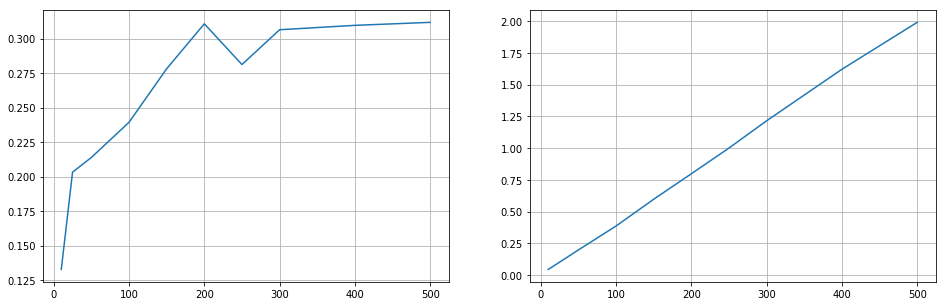
\includegraphics{output_23_0.png}

\(mejora = \frac{(energia(inicial) - energia(final))}{energia(inicial)}\)

Este número indica cuánto mejoró la solución final, en promedio,
respecto a la inicial en función de la temperatura inicial. Se puede
observar que a partir de una t0 de 200 se obtienen resultados
suficientemente aceptables. Duplicar la temperatura inicial significa
duplicar el tiempo de ejecución pero esto no se ve reflejado en una
mejora considerable en la calidad de la solución. Con 200 iteraciones ya
podemos considerar que la solución provista es buena.

\hypertarget{implementaciuxf3n-de-algoritmo-genuxe9tico-para-optimizar-la-ubicaciuxf3n-de-los-productos-en-el-almacuxe9n}{%
\section{Implementación de algoritmo genético para optimizar la
ubicación de los productos en el
almacén}\label{implementaciuxf3n-de-algoritmo-genuxe9tico-para-optimizar-la-ubicaciuxf3n-de-los-productos-en-el-almacuxe9n}}

En este problema se implementó un algoritmo genético para resolver el
problema de optimización de la ubicación de los productos en un layout
definido del almacen, de tal forma de optimizar el picking para un
conjunto de ordenes de productos habituales.

\hypertarget{anuxe1lisis-del-algoritmo-1}{%
\subsection{Análisis del algoritmo}\label{anuxe1lisis-del-algoritmo-1}}

El algoritmo es más específicamente un algoritmo genético con
permutaciones. Para la implementación fue necesario predifinir
diferentes etapas:

\begin{itemize}
\tightlist
\item
  \textbf{Individuos}:
\end{itemize}

A la hora de definir individuos se decidió hacer una especie de
``mapeo'' sobre el layout original. Es decir, si el layout es para 32
productos, cada individuo será una lista de números de 0 a 31 ordenados
de tal manera que el índice dará su posición. Por ejemplo, si un
individuo es {[}5, 2, 4, 0, 1, 3{]} el producto 5 estará ubicado donde
antes estaba el producto 0.

\begin{itemize}
\tightlist
\item
  \textbf{Función de fitness}:
\end{itemize}

Para calcular el fitness de un determinado individuo, se realiza un
\textbf{recocido simulado} (ya implementado en el ejercicio anterior)
para cada orden en el conjunto de órdenes habituales, para las cuales se
desea optimizar la ubicación de los productos. Si recordamos, la función
donde se implementó el recocido simulado recibe como parámetros la lista
de productos a recolectar, la temperatura inicial, la función de
generación de vecinos y la heurística a utilizar. Debido a que el
objetivo del algoritmo genético es justamente cambiar la ubicación de
los productos en el almacen, y el recocido simulado se ejecuta para el
layout original, en lugar de pasar el número de producto en la
secuencia, se pasa su índice en la lista (que es en definitiva el lugar
donde se encuentra).

Entonces, para cada orden del conjunto se ejecuta el recocido simulado,
que a su vez ejecuta internamente el algoritmo \textbf{A}*. Como
resultado se obtiene el costo de camino para esa orden, dada el layout
que es el individuo, y con el picking optimizado por el recocido
simulado. En teoría, es el menor costo posible al buscar todos los
productos de la orden en éste layout.

El fitness final del individuo será un promedio de los costos para cada
orden.

\begin{itemize}
\tightlist
\item
  \textbf{Selección}:
\end{itemize}

A la hora de elegir un individuo de la población previo al
\emph{crossover}, se utilizó \textbf{roulette wheel selection}. La idea
general es que la selección es aleatoria pero los individuos tienen
mayor probabilidad de ser elegidos cuanto menor sea su \emph{fitness}
(recuerdese que lo que se desea es minimizar el costo de
\emph{picking}).

\begin{itemize}
\tightlist
\item
  \textbf{Crossover}:
\end{itemize}

Se eligió \textbf{cruce de orden} como procedimiento de cruce por ser
apto para algoritmos genéticos de permutación. Consiste en seleccionar
dos puntos de cruce al azar, se copian los elementos de los padres entre
los puntos de cruce, cruzados, y luego se copian los valores restantes a
partir del segundo corte, en orden, evitando duplicar valores.

\begin{itemize}
\tightlist
\item
  \textbf{Mutación}:
\end{itemize}

Se eligió \textbf{inserción} también por ser apto para el problema de
permutaciones. Consiste en elegir 2 genes al azar de la solución, se
mueve el segundo gen elegido a continuación del primero y el resto de
los genes se mueven a la derecha.

\begin{itemize}
\tightlist
\item
  \textbf{Condición de corte}:
\end{itemize}

La condición de corte del algoritmo es por cantidad de iteraciones
(generaciones), y no por convergencia.

\hypertarget{evaluaciuxf3n-de-rendimiento-del-algoritmo}{%
\subsection{Evaluación de rendimiento del
algoritmo}\label{evaluaciuxf3n-de-rendimiento-del-algoritmo}}

\hypertarget{reducciuxf3n-de-fitness}{%
\subsection{\texorpdfstring{Reducción de
\emph{fitness}}{Reducción de fitness}}\label{reducciuxf3n-de-fitness}}

La primer evaluación que se realizó, y más intuitiva, fue la reducción
del fitness del mejor individuo de la población a lo largo de las
generaciones (iteraciones) del algoritmo.

Se creó un conjunto de ordenes aleaorias (conjunto para el cuál se debe
optimizar el almacén), de tal forma que ciertos productos tengan una
mayor tendencia a aparecer. Esto es a modo de evaluación visual,
intuyendo que los productos que más se repiten tenderían a aparecer
ubicados más cercas de donde se comienza el \emph{picking}.

\begin{Shaded}
\begin{Highlighting}[]
\ImportTok{from}\NormalTok{ genetic }\ImportTok{import}\NormalTok{ genetic, generate_ind}
\ImportTok{from}\NormalTok{ matplotlib }\ImportTok{import}\NormalTok{ pyplot }\ImportTok{as}\NormalTok{ plt}
\ImportTok{from}\NormalTok{ random }\ImportTok{import}\NormalTok{ randint, choices}

\NormalTok{N_POB }\OperatorTok{=} \DecValTok{10} \CommentTok{# Cantidad de individuos en la población}
\NormalTok{MAX_LENGHT }\OperatorTok{=} \DecValTok{32} \CommentTok{# Cantidad de estanterías}
\NormalTok{T_0 }\OperatorTok{=} \DecValTok{200} \CommentTok{# Temperatura inicial a la que inicia el algoritmo de temple simulado}
\NormalTok{MAX_GEN }\OperatorTok{=} \DecValTok{50} \CommentTok{# Máxima cantidad de iteraciones a la que corta el algoritmo genético}
\end{Highlighting}
\end{Shaded}

\begin{Shaded}
\begin{Highlighting}[]
\NormalTok{conjunto }\OperatorTok{=}\NormalTok{ []}

\NormalTok{prob }\OperatorTok{=}\NormalTok{ []}

\NormalTok{estant }\OperatorTok{=}\NormalTok{ [i }\ControlFlowTok{for}\NormalTok{ i }\KeywordTok{in} \BuiltInTok{range}\NormalTok{(}\DecValTok{0}\NormalTok{, MAX_LENGHT)]}

\ControlFlowTok{for}\NormalTok{ i }\KeywordTok{in} \BuiltInTok{range}\NormalTok{(}\DecValTok{0}\NormalTok{, }\DecValTok{25}\NormalTok{):}
\NormalTok{    prob.append(}\FloatTok{0.1}\NormalTok{)}

\ControlFlowTok{for}\NormalTok{ i }\KeywordTok{in} \BuiltInTok{range}\NormalTok{(}\DecValTok{25}\NormalTok{, MAX_LENGHT):}
\NormalTok{    prob.append(}\FloatTok{0.5}\NormalTok{)}

\ControlFlowTok{for}\NormalTok{ i }\KeywordTok{in} \BuiltInTok{range}\NormalTok{(}\DecValTok{0}\NormalTok{, }\DecValTok{8}\NormalTok{):}
\NormalTok{    conjunto.append(choices(population}\OperatorTok{=}\NormalTok{estant, k}\OperatorTok{=}\NormalTok{randint(}\DecValTok{3}\NormalTok{, }\DecValTok{7}\NormalTok{), weights}\OperatorTok{=}\NormalTok{prob))}

\BuiltInTok{print}\NormalTok{(conjunto)}
\end{Highlighting}
\end{Shaded}

\begin{verbatim}
[[30, 30, 12, 24], [30, 25, 5, 31, 25, 19, 10], [18, 1, 27, 29, 30], [3, 14, 10, 27, 31], [8, 9, 31, 29, 22, 25], [13, 10, 17, 1, 29, 22], [28, 8, 27, 6], [29, 18, 29, 16, 25, 26, 23]]
\end{verbatim}

\begin{Shaded}
\begin{Highlighting}[]
\NormalTok{start }\OperatorTok{=}\NormalTok{ []}
\ControlFlowTok{for}\NormalTok{ i }\KeywordTok{in} \BuiltInTok{range}\NormalTok{(}\DecValTok{0}\NormalTok{, N_POB):}
\NormalTok{    start.append(generate_ind())}

\NormalTok{best, history }\OperatorTok{=}\NormalTok{ genetic(start, conjunto, hist}\OperatorTok{=}\VariableTok{True}\NormalTok{, status}\OperatorTok{=}\VariableTok{False}\NormalTok{)}
\BuiltInTok{print}\NormalTok{(best)}

\NormalTok{plt.plot(history)}
\NormalTok{plt.grid()}
\end{Highlighting}
\end{Shaded}

\begin{verbatim}
[[26, 8, 29, 20, 17, 24, 30, 4, 25, 18, 27, 13, 10, 15, 5, 7, 31, 9, 2, 28, 14, 21, 3, 11, 6, 19, 23, 1, 12, 16, 22, 0], 1.0]
\end{verbatim}

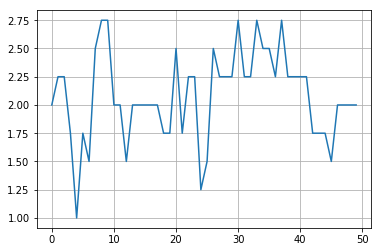
\includegraphics{output_9_1.png}

Como se puede observar en el gráfico, esta manera de evaluar no da
resultados conclusivos del funcionamiento del algoritmo, esto podría
deberse a que la diferencia de \emph{fitness} entre el estado inicial y
el óptimo no es la suficiente y al alcanzarse un mínimo este
\emph{fitness} comienza a oscilar.

\hypertarget{comparaciuxf3n-de-costos-con-layout-optimizado-y-sin-optimizar}{%
\subsection{Comparación de costos con layout optimizado y sin
optimizar}\label{comparaciuxf3n-de-costos-con-layout-optimizado-y-sin-optimizar}}

Dado que el análisis anterior no brinda resultados determinantes sobre
el rendimiento y funcionamiento del algoritmo, se buscó otra forma de
verificar que el algoritmo efectivamente funciona.

Se plantea ejecutar el recocido simulado para una determinada orden de
productos de tal forma de optimizar la secuencia del \emph{picking} esté
optimizada para el layout original del almacén. Luego ejecutar el
algoritmo genético para obtener el layout óptimo para dicha orden de
productos. Y por último, ejecutar el recocido simulado para la misma
orden pero esta vez con el layout del almacén optimizado.

\begin{Shaded}
\begin{Highlighting}[]
\ImportTok{from}\NormalTok{ simulated_annealing }\ImportTok{import}\NormalTok{ map_to_coord, temple_simulado, neighbours_annealing, distance}
\end{Highlighting}
\end{Shaded}

\begin{Shaded}
\begin{Highlighting}[]
\NormalTok{cost0 }\OperatorTok{=}\NormalTok{ []}
\NormalTok{cost1 }\OperatorTok{=}\NormalTok{ []}

\ControlFlowTok{for}\NormalTok{ orden }\KeywordTok{in}\NormalTok{ conjunto:}
\NormalTok{    coordenadas }\OperatorTok{=}\NormalTok{ map_to_coord(orden)}
\NormalTok{    _, costo }\OperatorTok{=}\NormalTok{ temple_simulado(coordenadas, }\DecValTok{200}\NormalTok{, neighbours_annealing, distance)}
\NormalTok{    cost0.append(costo)}
    
    \CommentTok{# Generación de población inicial}
\NormalTok{    start }\OperatorTok{=}\NormalTok{ []}
    \ControlFlowTok{for}\NormalTok{ i }\KeywordTok{in} \BuiltInTok{range}\NormalTok{(}\DecValTok{0}\NormalTok{, N_POB):}
\NormalTok{        start.append(generate_ind())}
    
\NormalTok{    new_layout, _ }\OperatorTok{=}\NormalTok{ genetic(start, [orden], status}\OperatorTok{=}\VariableTok{False}\NormalTok{)}
    
\NormalTok{    orden_estant }\OperatorTok{=}\NormalTok{ []}
    \ControlFlowTok{for}\NormalTok{ prod }\KeywordTok{in}\NormalTok{ orden:}
\NormalTok{        orden_estant.append(new_layout.index(prod))}
    
\NormalTok{    coordenadas }\OperatorTok{=}\NormalTok{ map_to_coord(orden_estant)}
\NormalTok{    _, costo }\OperatorTok{=}\NormalTok{ temple_simulado(coordenadas, }\DecValTok{200}\NormalTok{, neighbours_annealing, distance)}
\NormalTok{    cost1.append(costo)}
    
\end{Highlighting}
\end{Shaded}

\begin{Shaded}
\begin{Highlighting}[]
\NormalTok{plt.plot(cost0, label}\OperatorTok{=}\StringTok{"costo con layout sin optimizar"}\NormalTok{)}
\NormalTok{plt.plot(cost1, label}\OperatorTok{=}\StringTok{"costo con layout optimizado"}\NormalTok{)}
\NormalTok{plt.grid()}
\end{Highlighting}
\end{Shaded}

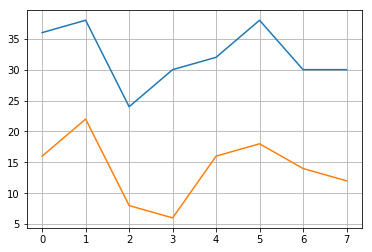
\includegraphics{output_15_0.png}

\begin{Shaded}
\begin{Highlighting}[]
\NormalTok{avg }\OperatorTok{=} \DecValTok{0}
\ControlFlowTok{for}\NormalTok{ i, j }\KeywordTok{in} \BuiltInTok{zip}\NormalTok{(cost0, cost1):}
\NormalTok{    avg }\OperatorTok{+=}\NormalTok{ (i }\OperatorTok{-}\NormalTok{ j) }\OperatorTok{/}\NormalTok{ i}
\NormalTok{avg }\OperatorTok{=}\NormalTok{ avg }\OperatorTok{*} \DecValTok{100} \OperatorTok{/} \BuiltInTok{len}\NormalTok{(cost0)}

\BuiltInTok{print}\NormalTok{(avg)}
\end{Highlighting}
\end{Shaded}

\begin{verbatim}
56.275638544891635
\end{verbatim}

En el gráfico anterior pueden observarse diferencias claras al optimizar
la ubicación de los productos en el almacen para un conjunto de ordenes,
por lo que puede concluirse que el algoritmo está funcionando
correctamente, reduciendo costos en aproximadamente \textbf{56,27\%}.

\hypertarget{anuxe1lisis-de-la-probabilidad-de-mutaciuxf3n}{%
\subsection{Análisis de la probabilidad de
mutación}\label{anuxe1lisis-de-la-probabilidad-de-mutaciuxf3n}}

En \href{./genetic-test.py}{genetic-test.py} se realiza un análisis para
encontrar un valor aceptable de probabilidad de mutación. Esto se
obtiene ejecutando el análisis anterior y comparando la reducción
promedio obtenida del conjunto de ordenes.

Los resultados obtenidos son los de la gráfica:

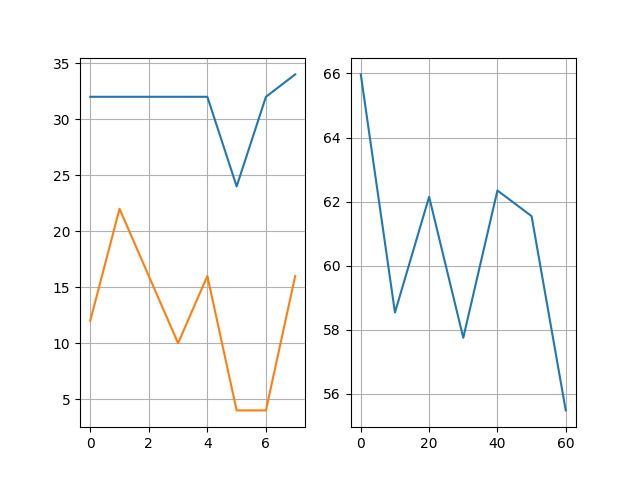
\includegraphics{genetic_test.png}

\hypertarget{implementaciuxf3n-de-algoritmo-de-satisfacciuxf3n-de-restricciones}{%
\section{Implementación de algoritmo de satisfacción de
restricciones}\label{implementaciuxf3n-de-algoritmo-de-satisfacciuxf3n-de-restricciones}}

Se implementó un algoritmo de \emph{backtracking} para resolver el
problema de satisfacción de restricciones, más especificamente, de
\emph{scheduling}.

\hypertarget{modelado-del-problema-1}{%
\subsection{Modelado del problema}\label{modelado-del-problema-1}}

El problema consiste en una determinada cantidad de tareas que deben
realizarse, donde cada una demanda un determinado tiempo:

\begin{Shaded}
\begin{Highlighting}[]
\NormalTok{T }\OperatorTok{=}\NormalTok{ \{}\StringTok{"d0"}\NormalTok{: }\DecValTok{40}\NormalTok{, }\StringTok{"d1"}\NormalTok{:}\DecValTok{20}\NormalTok{, }\StringTok{"d2"}\NormalTok{:}\DecValTok{25}\NormalTok{, }\StringTok{"d3"}\NormalTok{:}\DecValTok{10}\NormalTok{, }\StringTok{"d4"}\NormalTok{:}\DecValTok{30}\NormalTok{\}}
\end{Highlighting}
\end{Shaded}

Como restricción global a la hora de asignar valores, se considera desde
un principio (acotando el dominio de las variables) que el proceso total
debe finalizarse en un tiempo menor a \emph{DLINE}. Además, el tiempo se
discretizó en intervalos con valor \emph{STEP}.

\begin{Shaded}
\begin{Highlighting}[]
\NormalTok{DLINE }\OperatorTok{=} \DecValTok{150}
\NormalTok{STEP }\OperatorTok{=} \DecValTok{5}
\end{Highlighting}
\end{Shaded}

Por lo tando, la asignación de los valores en el dominio de cada
variable es de la forma:

\begin{Shaded}
\begin{Highlighting}[]
\NormalTok{D }\OperatorTok{=}\NormalTok{ \{\}}
\ControlFlowTok{for}\NormalTok{ i }\KeywordTok{in}\NormalTok{ T.keys():}
\NormalTok{    D[i] }\OperatorTok{=} \BuiltInTok{list}\NormalTok{(}\BuiltInTok{range}\NormalTok{(}\DecValTok{0}\NormalTok{, DLINE}\OperatorTok{-}\NormalTok{T[i], STEP))}
\end{Highlighting}
\end{Shaded}

Luego se crea un diccionario vacío que contendra las futuras
asignaciones del algoritmo, y se elige una variable aleatoria no
asignada (por ser la inicial se elige aleatoriamente de entre todo el
conjunto de variables).

\begin{Shaded}
\begin{Highlighting}[]
\ImportTok{from}\NormalTok{ backtracking }\ImportTok{import}\NormalTok{ selection}

\NormalTok{assign }\OperatorTok{=}\NormalTok{ \{\}}
\BuiltInTok{print}\NormalTok{(selection(D, assign))}
\end{Highlighting}
\end{Shaded}

\begin{verbatim}
d0
\end{verbatim}

Es importante tener en cuenta que a la hora de elegir una variable no
asignada se puede implementar alguna heurística como \emph{mínimos
valores restantes}. En la práctica esto no se realizó.

\hypertarget{restricciones-binarias-de-precedencia}{%
\subsubsection{Restricciones binarias de
precedencia}\label{restricciones-binarias-de-precedencia}}

Las restricciones binarias se describen \emph{harcodeando} la relación
de precedencia entre las distintas variables, teniendo en cuenta el
orden.

A continuación se plantea un grafo de restricciones sencillos para que
puede verificarse visualmente la solución.

\begin{Shaded}
\begin{Highlighting}[]
\NormalTok{R2 }\OperatorTok{=}\NormalTok{ \{}
    \StringTok{"d0"}\NormalTok{:[(}\StringTok{"d0"}\NormalTok{, }\StringTok{"d1"}\NormalTok{), (}\StringTok{"d0"}\NormalTok{, }\StringTok{"d2"}\NormalTok{)],}
    \StringTok{"d1"}\NormalTok{:[(}\StringTok{"d0"}\NormalTok{, }\StringTok{"d1"}\NormalTok{), (}\StringTok{"d1"}\NormalTok{, }\StringTok{"d3"}\NormalTok{)],}
    \StringTok{"d2"}\NormalTok{:[(}\StringTok{"d0"}\NormalTok{, }\StringTok{"d2"}\NormalTok{), (}\StringTok{"d2"}\NormalTok{, }\StringTok{"d4"}\NormalTok{)],}
    \StringTok{"d3"}\NormalTok{:[(}\StringTok{"d1"}\NormalTok{, }\StringTok{"d3"}\NormalTok{), (}\StringTok{"d3"}\NormalTok{, }\StringTok{"d4"}\NormalTok{)],}
    \StringTok{"d4"}\NormalTok{:[(}\StringTok{"d3"}\NormalTok{, }\StringTok{"d4"}\NormalTok{), (}\StringTok{"d2"}\NormalTok{, }\StringTok{"d4"}\NormalTok{)]}
\NormalTok{\}}
\end{Highlighting}
\end{Shaded}

\hypertarget{restricciones-binarias-de-recursos}{%
\subsubsection{Restricciones binarias de
recursos}\label{restricciones-binarias-de-recursos}}

Cada tarea ocupa máquinas que están disponibles en cantidad limitada,
por lo tanto no pueden ejecutarse tareas que requieren de la misma
máquina en paralelo.

Este tipo de restricciones se describen asignando una lista de máquinas
requeridas a cada tarea.

\begin{Shaded}
\begin{Highlighting}[]
\NormalTok{M }\OperatorTok{=}\NormalTok{ \{}
    \StringTok{"d0"}\NormalTok{:[}\StringTok{"m1"}\NormalTok{, }\StringTok{"m3"}\NormalTok{],}
    \StringTok{"d1"}\NormalTok{:[}\StringTok{"m2"}\NormalTok{, }\StringTok{"m4"}\NormalTok{],}
    \StringTok{"d2"}\NormalTok{:[}\StringTok{"m0"}\NormalTok{],}
    \StringTok{"d3"}\NormalTok{:[}\StringTok{"m0"}\NormalTok{, }\StringTok{"m2"}\NormalTok{, }\StringTok{"m3"}\NormalTok{],}
    \StringTok{"d4"}\NormalTok{:[}\StringTok{"m0"}\NormalTok{, }\StringTok{"m4"}\NormalTok{]}
\NormalTok{\}}
\end{Highlighting}
\end{Shaded}

\hypertarget{soluciuxf3n}{%
\subsubsection{Solución}\label{soluciuxf3n}}

La solución será el diccionario de tareas, con el valor de tiempo
inicial en el que se ejecutará cada una.

\begin{Shaded}
\begin{Highlighting}[]
\ImportTok{from}\NormalTok{ backtracking }\ImportTok{import}\NormalTok{ backtrack}

\BuiltInTok{print}\NormalTok{(backtrack(T, assign, D, R2, M))}
\end{Highlighting}
\end{Shaded}

\begin{verbatim}
{'d4': 75, 'd3': 60, 'd2': 40, 'd0': 0, 'd1': 40}
\end{verbatim}

\hypertarget{conclusiuxf3n-1}{%
\subsubsection{Conclusión}\label{conclusiuxf3n-1}}

El algoritmo por ser \emph{backtracking} básico, sin la implementación
de algún otro algoritmo para analizar arco consistencia como
\emph{AC-3}, es muy ineficiente pero da soluciones correctas.

\end{document}
